\chapter{Complex event processing}
	\label{chap:cep}
	\section{Intro of the Complex Event Processing}
		In our hierarchical runtime verification project, the top level of modelling is done in an event pattern language.
		This event pattern language (vepl) can be translated to timed regular expressions, which can be translated to 
		timed event automatons. We'll use this to implement the event processor. 
	\section{Background}
		\subsection{VEPL}
			TODO add a reference to David Istvans work
			
			TODO define event.
			
			TODO define complex event processing
			
			The used formalism to define event patterns is the VEPL. A brief overview to this language:
			
			
			Operators

			\begin{figure}[h]
			\centering
			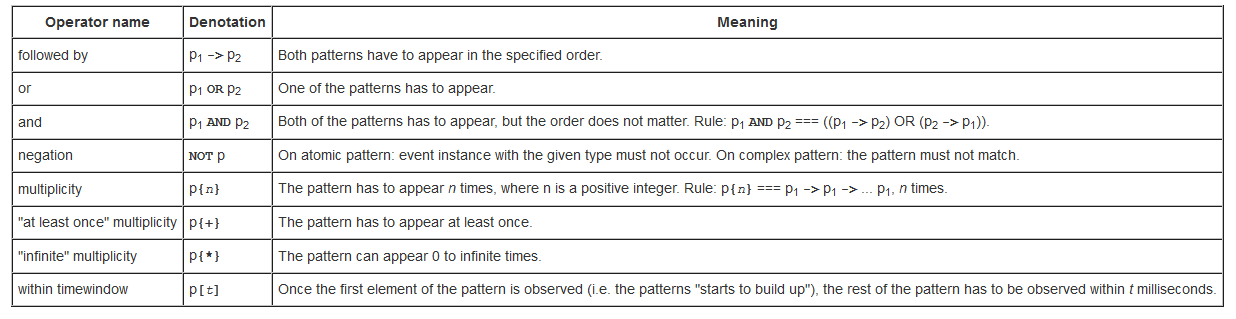
\includegraphics[width=0.5\linewidth]{include/figures/chapter_5/viatracepoperators}
			\caption{Operators of the VIATRA CEP}
			\label{fig:cep:viatracepoperators}
			\end{figure}			
			
			
		\subsection{Timed Regular Expression}
			\begin{dfn}
				Timed Regular Expressions over an alphabet $\Sigma$ (also referred to as $\Sigma$-expressions)
				are defined using the following families of rules.
				\begin{enumerate}
					\item{a for every letter $a \in \Sigma$ and the special symbol $\varepsilon$ are expressions}
					\item{If $\varphi, \varphi_1, \varphi_2$ are $\Sigma$-expressions and I is an integer-bounder iterval then
					$\langle\varphi_I\rangle, \varphi_1 \cdot \varphi_2, \varphi_1 \vee \varphi_2,$ and $\varphi^\ast$ are $\Sigma$-expressions.}
					\item{If $\varphi, \varphi_1$ and $\varphi_2$ are $\Sigma$-expressions then $\varphi_1 \circ \varphi_2, \varphi^\circledast$ are
					$\Sigma$-expressions}
.					\item{If $\varphi_1$ and $\varphi_2$ are $\Sigma$-expressions, $\varphi_0$ is a $\Sigma_0$-expression
					for some alphabet $\Sigma_0$, and $\Theta$ : $\Sigma_0 \rightarrow \Sigma$ is
					a renaming, then $\varphi_1 \wedge \varphi_2$ and $\Theta(\varphi_0)$ are $\Sigma$-expressions}
				\end{enumerate}
			\end{dfn}
			
		
		\subsection{Event Automaton}
			% informal definition
			An Event Automaton is a non-deterministic finite-state automaton whose alphabet consists
			of parametric events and whose transitions may be labelled with guards and assignments
			
			% formal definition
			\begin{dfn}
				An EA
				$\langle Q,\mathcal{A},\delta, q_0, F \rangle$ is a tuple where Q is a finite set of states, 
				$\mathcal{A} \subseteq Event$ is a finite alphabet,
				$\delta \in (Q \times \mathcal{A} \times Guard \times Assign \times Q)$ is a finite set of transitions, 
				$q_0 \in Q$ is an initial state, and 
				$F \subseteq Q$ is a set of final states.
			\end{dfn}
			
		\subsection{Timed Event Automaton}
			% stuff about the calendar
			% informal definition of the calendar?
			In discrete event simulation, a calendar (also called event list) is a data structure that
			stores future events and the times at which these events are scheduled to occur
			
			% Formal definition of the calendar
				% \begin{dfn}
				% A calendar is a finite set (or multiset) of the form $C = \{ \langle e_1, t_1\rangle \, \dots ,\langle e_n, t_n\rangle \}$
				% where each $e_i$ is an event and $t_i$ is the time when event $e_i$ is scheduled to occur. All $t_i$s are real numbers.
				% We denote by min(C) the smallest number among $\{t_1,\dots ,t_n \}$ (with min(C) = $+\infty$ if C is empty)
				% Given a real u, we denote by $Ev_u(C)$ the subset of C that contains all events scheduled at time u:
				% $Ev_u(C) = \{ \langle e_i, t_i \rangle  | t_i = u \wedge \langle e_i , t_i \rangle \in C \} $
				% \end{dfn}
			% stuff about the calender automaton
				
				
		\subsection{Our Formalism}
			TimedZone is a tuple $\langle StartState, EndZones, TimeoutValue, StateMoveTo  \rangle$
			
			If a token enters a state, and there is a TimeZone whose StartState is the state, and it doesn't enter a state which is one of the EndStates before the timeout, the token'll be moved to the StateMoveTo.
			
			Our Automaton = $\langle EventAutomaton, TZ \rangle$ where TZ is a Set of TimedZones
	\section{Examples of Event Processing}
 
		\subsection{varphile System}
			\subsubsection{Problem}
				varphile system - A file shouldn't be read when it has been opened for writing, and shouldn't be written, when opened for reading. 
				A file shouldn't be opened for writing and reading without a close event between the two different opens.
				The possible parametrized events are : Open(file, mode), Close(file), Read(file), Write(file). Mode is either "R" or "W" which stands for Read and Write respectively.
			\subsubsection{Solution}
				We are looking for these patterns : 
				
				open(f,"W") $\rightarrow$ NOT close(f)$\{\ast\}$ $\rightarrow$ open(f,"R");
				
				open(f,"R") $\rightarrow$ NOT close(f)$\{\ast\}$ $\rightarrow$ open(f,"W");
				
				open(f,"W") $\rightarrow$ NOT close(f)$\{\ast\}$ $\rightarrow$ read(f);
				
				open(f,"R") $\rightarrow$ NOT close(f)$\{\ast\}$ $\rightarrow$ write(f);
				
				\begin{figure}[h]
				\centering
				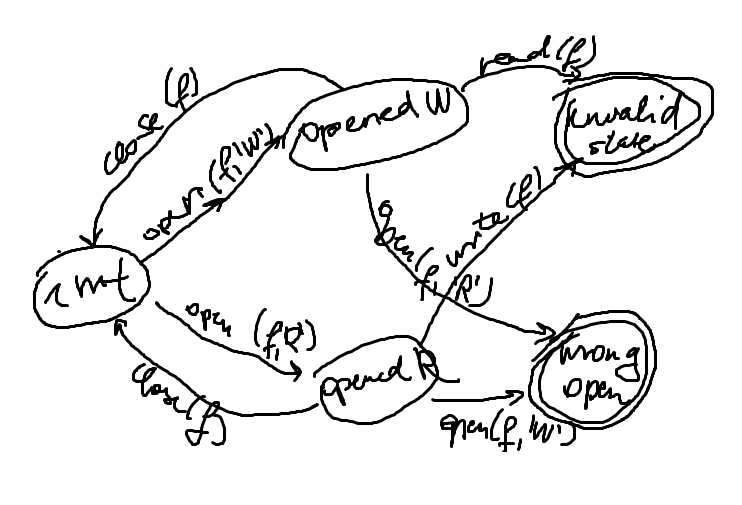
\includegraphics[width=0.5\linewidth]{include/figures/chapter_5/fileautomaton}
				\caption{Automaton of the file example}
				\label{fig:cep:fileautomaton}
				\end{figure}

		
		
		\subsection{Mars Rover Tasking - Two phase locking}
			\subsubsection{Problem}
				In concurrent systems the avoidance of deadlocks and livelocks are an utmost importance.
				To solve this problem, one of the many patterns is  the two phase locking - which can be defined by two rules.
				These rules are : 
				\begin{enumerate}
					\item{Every task must allocate the resources in a given order.}
					\item{If a task releases a resource, it can't allocate anymore}
				\end{enumerate}
			\subsubsection{Solution}
				Since our implementation doesn't support guards (yet) 

	\section{Implementation}
		\subsection{Metamodel}
		
			\begin{figure}[h]
			\centering
			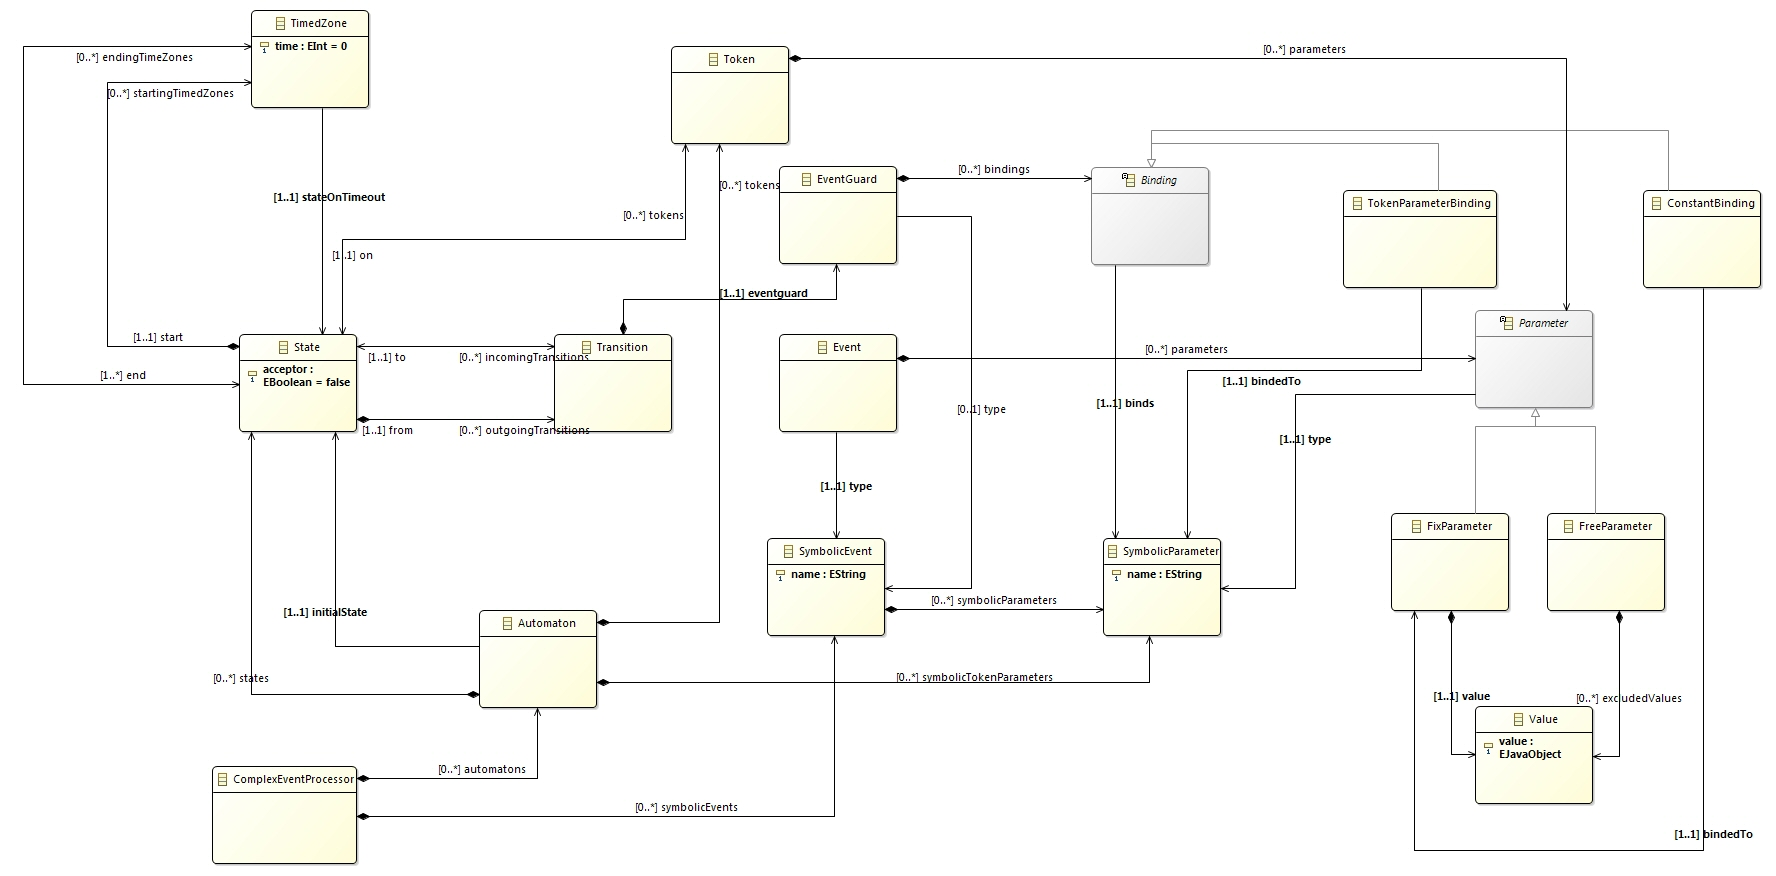
\includegraphics[width=0.9\linewidth]{include/figures/chapter_5/model}
			\caption{Automaton of the file example}
			\label{fig:cep:model}
			\end{figure}
		%image
		Nyilvan ide mjd kisebb, mutatosabb, es kevesebb dolgot tartalmazo abra kell, meg nemi magyarazat
		\subsection{Executor}
			The algorithm first searches for all the activated transitions.
			If it finds an activated transition, it iterates over the tokens which are on the state. The first token with matching (non-confronting)
			parameter list will be split to the next state if there are new parameter bindings from the event, or moved if there are no new bindings.
			If a token enters an acceptor state it'll 
			next state 